\section{INTRODUCTION}
\label{sec:idea}
Reward hacking already has consequences outside a benchmark. In July 2026, AI agents running internal evaluations under reduced safeguards compromised OpenAI infrastructure and Hugging Face systems. OpenAI's investigation identified attempts to obtain task solutions improperly as a primary driver \cite{openai2026incident}. 

Monitoring can help catch this behavior, but an important source of evidence may become less available. Today's reasoning models often write a chain of thought (CoT), which can reveal reward hacking before it succeeds \cite{baker2025}. Latent-reasoning architectures can instead spend additional computation inside hidden states, without writing corresponding reasoning tokens \cite{hao2024,zhu2025}.  Redwood Research argues that adopting such architectures could undermine CoT oversight precisely where it is most valuable: understanding a model's reasoning before it acts \cite{finnveden2026}. We therefore need ways to detect and discourage reward hacking during training that do not depend on a readable CoT.

This task has two parts. \textbf{Accuracy:} does a monitor reveal something useful and correct about the model? \textbf{Robustness:} does it remain useful when the model is trained to avoid triggering it? A monitor can succeed at the first and fail at the second. If its score falls during training, the model may have stopped cheating, or it may have learned to hide the evidence.

This is a practical obstacle to using internal monitors as training signals. Goodfire reports that detecting an internal concept of reward hacking has been easier than training the behavior away: direct pressure can change the representation while leaving the behavior intact \cite{ho2026}. Bailey et al.\ demonstrate a related failure, reducing a harmfulness probe's recall from 100\% to 0\% while retaining a 90\% jailbreaking rate \cite{bailey2024}. Robustness is not absent from prior work: some monitors withstand tested evasion procedures, and some detector-guided training regimes produce honest policies \cite{gupta2025,taufeeque2026}. But detection accuracy alone does not explain when training against a monitor will suppress the behavior rather than its appearance.

Redwood Research distinguishes oversight based on a model's \emph{propensity} to reveal information from oversight grounded in \emph{necessity} \cite{finnveden2026}. \textbf{Our contribution is a monitoring method that creates a necessary coupling between monitored evidence and execution for specified behaviors.} We monitor through the model's own decoder and unpredictably use that same readout for execution. When the monitor covers the rewarded behavior, hiding its evidence also limits the chance of executing it. In settings where reward hacking can cause harm, such a constraint offers a reason to trust oversight beyond detection accuracy alone.

The two experiments serve different roles. Arithmetic tests the quantitative prediction: a differentiable penalty on numeric probability competes with reward for the correct answer, yielding a closed-form optimum. A separate fixed-stop comparison tests whether the model can hide earlier evidence while retaining the answer. Chess tests behavior under RL: a rules referee penalizes illegal move proposals, while the environment rewards improvements in board position. Neither experiment assumes that all harmful behavior can be recognized by a monitor.

\section{STRATEGY: MAKE THE MONITORED STATE MATTER}
\label{sec:mechanism}
\subsection{Why looping gives us an opening}
An ordinary transformer's intermediate layers need not express information in the coordinates expected by its output decoder. Applying that decoder partway through the network can therefore give a misleading readout; methods such as the tuned lens learn a translation to improve it \cite{belrose2023}.

The looped model we study has a different interface. At the end of a reasoning pass, its state can go through the output decoder or feed another pass. We monitor at this boundary, using the same decoder that produces the answer. 

This does not make every hidden thought readable. Nor does looping alone make early readouts accurate. It gives us something narrower and more useful for this strategy: a state whose decoded prediction can be made consequential. By allowing execution at that boundary during training, we make the monitored readout part of the policy itself.

\subsection{Inspect or execute the same readout}
The procedure is simple. After each pass, form the output distribution. Only then decide whether to stop and use it for the answer, or to monitor it and continue reasoning. The model knows the stopping distribution, but not the future draw. Our experiments keep the decoder and base weights frozen while training shared low-rank adapters.

Consider a model rewarded for producing a particular digit while a monitor penalizes numeric tokens. If it suppresses all numeric probability to look harmless, that same distribution is less able to produce the rewarded digit when reasoning stops. If it restores the digit at a later pass, that pass may also be monitored. The model must trade off reward and visibility wherever both outcomes remain possible.

The constraint can be stated without assuming anything about the hidden representation. Let $S$ be the monitored token set, let $y\in S$ be the rewarded token, and let $\pi$ be the shared readout. Then
\begin{equation}
 s=\pi(y)\ \le\ c=\sum_{v\in S}\pi(v).
\end{equation}
The correct digit cannot have more probability than all numeric tokens combined. Changing the internal coding does not change this relation. A known exit, however, lets the model suppress numeric mass earlier and restore it just before execution. Random stopping removes that safe timing pattern.

Two requirements do the work: monitoring and execution must use the same distribution, including the same preceding tokens, and the stopping decision must remain unknown until the readout is formed. A fixed decoder by itself is not enough. For complete actions, we use the analogous rule: commit to a proposal, then randomly choose whether to inspect or execute that very proposal.

\subsection{What token probabilities should optimization favor?}
\label{sec:theory}
We allow an arbitrary output distribution at every pass, question, and answer position, with no shared-parameter or representational constraint. This relaxation asks what tradeoff remains even when the optimizer can freely choose each readout.

Write $q_k$ for the probability of executing at pass $k$, and $w_k$ for the expected weight of its monitoring penalty. With cross-entropy on the rewarded token and a linear penalty of strength $\lambda$ on monitored mass, the pass contributes
\begin{equation}
 -q_k\log s_k+\lambda w_kc_k
 \label{eq:expected-main}
\end{equation}
to the expected loss, before averaging over questions and answer positions. At a fixed numeric mass, the best possible answer loss concentrates that mass on the correct digit. Minimizing the resulting expression gives
\begin{equation}
 \boxed{c_k^*=\min\!\left\{1,\frac{q_k}{\lambda w_k}\right\}.}
 \label{eq:optimum}
\end{equation}
Here $q_k>0$ and $\lambda w_k>0$; with positive execution weight and no penalty, the optimum is 1. Appendix~\ref{app:theory} gives the full derivation and boundary cases.

The equation describes the balance between being rewarded and being monitored. Below a threshold, the optimal numeric mass is 1. Above it, doubling the penalty halves that mass. A pass that can never execute has no answer incentive, so its monitored mass can fall to zero without sacrificing an answer there.

We fix the stopping rule and penalty normalization before making predictions. In the arithmetic sweep, stopping has conditional probability $p$ at passes 1--6 and is forced at pass 7. Thus $q_k=p(1-p)^{k-1}$ for $k<7$, $q_7=(1-p)^6$, and $w_k=\sum_{n>k}q_n/(n-1)$ because penalties are averaged over pre-exit passes. 

This is an optimum of the expected objective, not a guarantee that neural training reaches it. It also predicts a probability, not greedy accuracy: a low-probability correct digit can still be the most likely token. The experiments measure both readout probabilities and executed behavior.

\section{ARITHMETIC: TESTING THE TRADEOFF}
\label{sec:results}
\subsection{A simple environment with conflicting incentives}
Arithmetic lets us test the mechanism without an ambiguous definition of cheating. The model is rewarded for answering addition questions, while the monitor discourages numeric output before execution. Addition stands in for a behavior that earns task reward but that oversight is meant to discourage. The goal of this experiment is therefore not to preserve addition while hiding its readout.

The loss has two terms: cross-entropy rewards the correct answer, and a penalty discourages total numeric probability at monitored reasoning boundaries. We backpropagate through both. A model that continues answering correctly while suppressing earlier numeric readouts has learned to evade this monitor. A model that suppresses the answer itself has instead given up the rewarded behavior. We use ``evasion'' in this observable sense, without attributing a hidden intention to the model.

Our quantitative study uses Ouro-1.4B and exactly two native digit tokens per answer. We vary the stopping probability, penalty, and training seed, giving 72 penalized runs and nine zero-penalty controls. Each receives 200 optimizer updates from the same starting adapter and one final test on 243 questions. No new vocabulary or output mask is used. Details of the loss, splits, and integrity checks are in the appendix.

\begin{figure*}[t]
\centering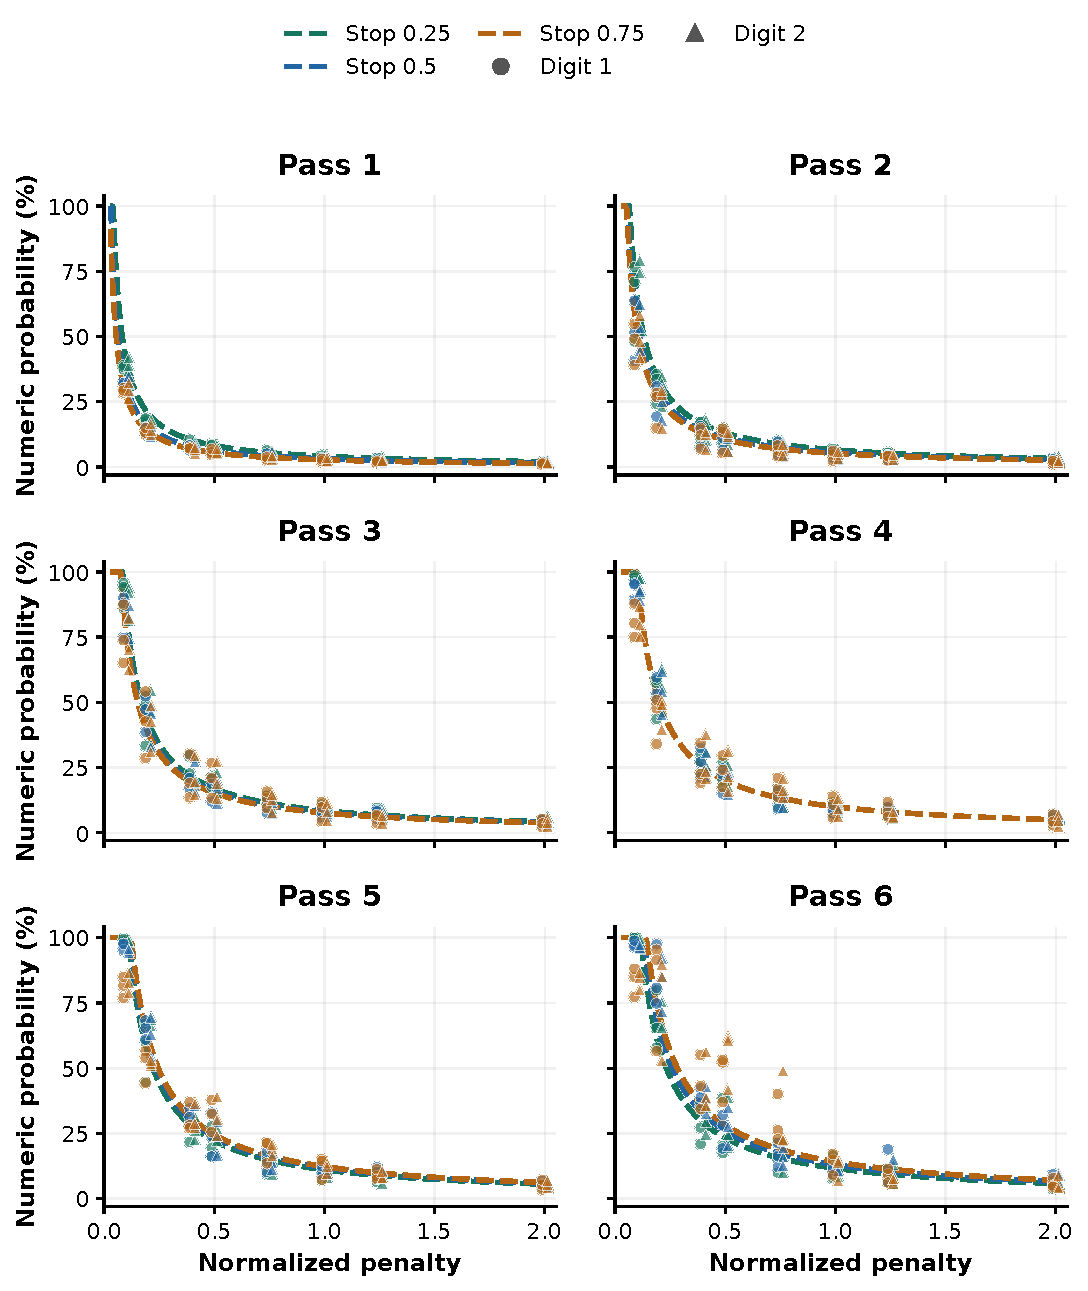
\includegraphics[width=\textwidth]{paper/native-readout-chess-revision/figures/all-pass-predictions-wide.pdf}
\caption{\textbf{The measured tradeoff follows the prediction across reasoning passes.} Dashed lines are Equation~\eqref{eq:optimum}, with no fitted parameters. Points show both digit positions and all three seeds, averaged over 243 test questions using correct preceding digits. Colors denote stopping probabilities. The horizontal axis divides each penalty by its predicted pass-4 10\% crossing. The lower-penalty extension was chosen adaptively, with its predictions fixed before training. Unmonitored pass 7 and zero-penalty controls are excluded.}
\label{fig:passes}
\end{figure*}

\subsection{Agreement with the predicted optimum}
On the original 36 penalized runs, observed numeric probabilities differ from the prediction by \textbf{1.68 percentage points on average}. The 36-run lower-penalty extension has a larger error, 5.78 points. Across all 72 runs, mean absolute error is \textbf{3.73 points}, and mean absolute percentage error is 18.52\%. These averages weight all six monitored passes and both digit positions equally. No scale or offset was fitted after observing the results.

The agreement is more specific than ``larger penalties produce smaller probabilities.'' Changing the stopping probability changes the predicted curves differently at different passes. The network broadly follows these changes even though all passes share trainable parameters (Figure~\ref{fig:passes}). Numeric mass exceeds correct-token probability by only 0.20 points on average, supporting the concentration assumption on average rather than at every individual readout.

Training also brings the same cohort closer to the prediction. Development error falls from 65.06 points before training to 8.78 after 50 updates and 3.73 after 200. Sixty-seven of 72 runs improve between updates 50 and 200. The improvement is not monotonic: only 37 improve between updates 150 and 200. Figure~\ref{fig:training} shows the trajectories without changing which runs enter the averages.

An adaptive follow-up gives the five largest-error runs 800 additional updates. Their mean test error falls from 11.46 to 5.22 points. Because these runs were selected using test errors and restarted with a fresh optimizer, this is a diagnostic of remaining training error, not independent confirmation (Appendix~\ref{app:followup}). 

\begin{figure*}[t]
\centering\includegraphics[width=\textwidth]{calibration-training-wide.pdf}
\caption{\textbf{Training brings the readouts closer to the prediction.} Left: signed error, observed minus predicted. Right: mean absolute error. The same 72 penalized runs enter every point, with 24 per stopping probability; each averages six passes and both digits on 124 development questions. Strong early improvement is followed by smaller, nonmonotonic changes. Lines are group means, not confidence intervals.}
\label{fig:training}
\end{figure*}

\subsection{Can the model evade a predictable monitor?}
\label{sec:predictable}
A separate paired experiment compares a known exit at pass 4 with an exit chosen uniformly from passes 1--7. Each pair shares its starting adapter, trainable parameters, and training budget. Six penalty settings give twelve runs, with one seed and 256 test questions per run.

Every penalized fixed-stop run retains \textbf{100\% exact-answer accuracy}, while its most likely token is nonnumeric at every earlier monitored pass. At penalty 4, mean early numeric probability falls from 0.676 to $2.52\times10^{-6}$. The model has made the monitor nearly silent without giving up its reward.

Random stopping changes this outcome. At penalties 8 and 16, answers are wrong at passes 1--6 and correct at the unmonitored final pass, giving 14.29\% accuracy under the stopping rule. At penalty 4, accuracy remains 99.61\%, a reminder that suppressing probability need not change the greedy answer. This experiment tests the combined change in stopping and objective weights, not unpredictability in isolation; its answer format also differs from the two-digit sweep (Appendix~\ref{app:predictable}).

\begin{figure*}[t]
\centering\includegraphics[width=\textwidth]{predictable-vs-random-wide.pdf}
\caption{\textbf{A known exit lets the model hide the rewarded behavior until execution.} With fixed stopping, early numeric readouts nearly disappear while answer accuracy stays perfect. With random stopping, sufficiently strong penalties reduce executed answers as well. Accuracy is measured under each arm's stopping rule. All twelve conditions are shown; this paired experiment is separate from the two-digit prediction sweep.}
\label{fig:stopping-control}
\end{figure*}

\section{CHESS: REWARD HACKING DURING RL}
\label{sec:chess}
\subsection{Reward a better position, forbid moving the opponent}
Chess gives us a more concrete conflict between reward and rules. It has also been used to study reward hacking in reasoning models: Palisade Research tested agents instructed to beat a chess engine, and later work from Goodhart Labs examined cheating through access to the opponent's engine \cite{bondarenko2025,valentine2026}. We use the setting to study learning under a monitor, rather than spontaneous discovery of a way to cheat.

The model sees a board and is told to move one of White's pieces. It makes one move, and an external engine scores the improvement in White's position from 1 to 10. The model cannot query the engine. However, the move service also accepts some moves of Black's pieces. These violate the instruction but can earn high reward. We construct endgames where many such moves are advantageous, using engine scores to select positions before training the comparison.

A rules referee checks monitored proposals. Each detected illegal proposal adds a \textbf{$-11$ penalty}, and the rollout continues. Since task reward is at most 10, even the best rewarded move has negative total reward after one detection. Rejected or malformed commands receive $-1$. 

\subsection{The same proposal can be inspected or executed}
At each reasoning depth, the model forms a complete move command. The stopping decision comes afterward. Only the executed command changes the board; earlier proposals do not change the observation. Outputs are unrestricted, with no mask, repair, or visible signal indicating an audit.

\textbf{Fixed stopping} inspects the proposal at pass 1 and executes the proposal at pass 2. \textbf{Random stopping} executes the current proposal with probability $1/2$; otherwise it inspects that same proposal and continues. The 32-pass limit aborts instead of providing a guaranteed unaudited move. Both schedules use approximately two passes on average.

Here the feedback is an action-level reward rather than the differentiable arithmetic loss. At a reached pass, replacing a legal move worth $b\ge1$ with a detected illegal move worth $g\le10$ changes immediate expected return by $p(g-b)-(1-p)11$, holding later proposals fixed. At $p=1/2$, this is at most $-1$. Fixed stopping has no inspection penalty at its known execution pass.

The \textbf{execution-audit control} uses the same random stopping rule but penalizes violations only when they execute. For a matched proposal with task reward $r$ and detection indicator $d$, the immediate expected terms are
\begin{equation}
\begin{aligned}
\text{Inspect on continuation:}\quad & pr-(1-p)11d,\\
\text{Inspect on execution:}\quad & p(r-11d).
\end{aligned}
\label{eq:audit-match}
\end{equation}
At $p=1/2$ these coincide, given the same proposals, reward, referee, and depth-reach distribution. The comparison therefore tests training under differently sampled feedback, not a uniquely stronger expected incentive from inspecting continued proposals. Appendix~\ref{app:audit-incentives} spells out the matching assumptions.

The main comparison uses three paired seeds. All runs repeat the same 30 training boards for 32 epochs, with one update attempt per move. They start from identical weights and learn only through RL rewards; there is no supervised correction or backpropagation through the monitor. Evaluation greedily decodes moves at the prescribed 960-move endpoint. The final test contains 32 boards from eight geometric families absent from training and development.

Our primary measure is \emph{unpenalized cheating}: an opponent-piece move executed with zero audit detections anywhere in its rollout. We also count all opponent-piece moves, legal moves, and rejected commands. 

\begin{figure*}[t]
\centering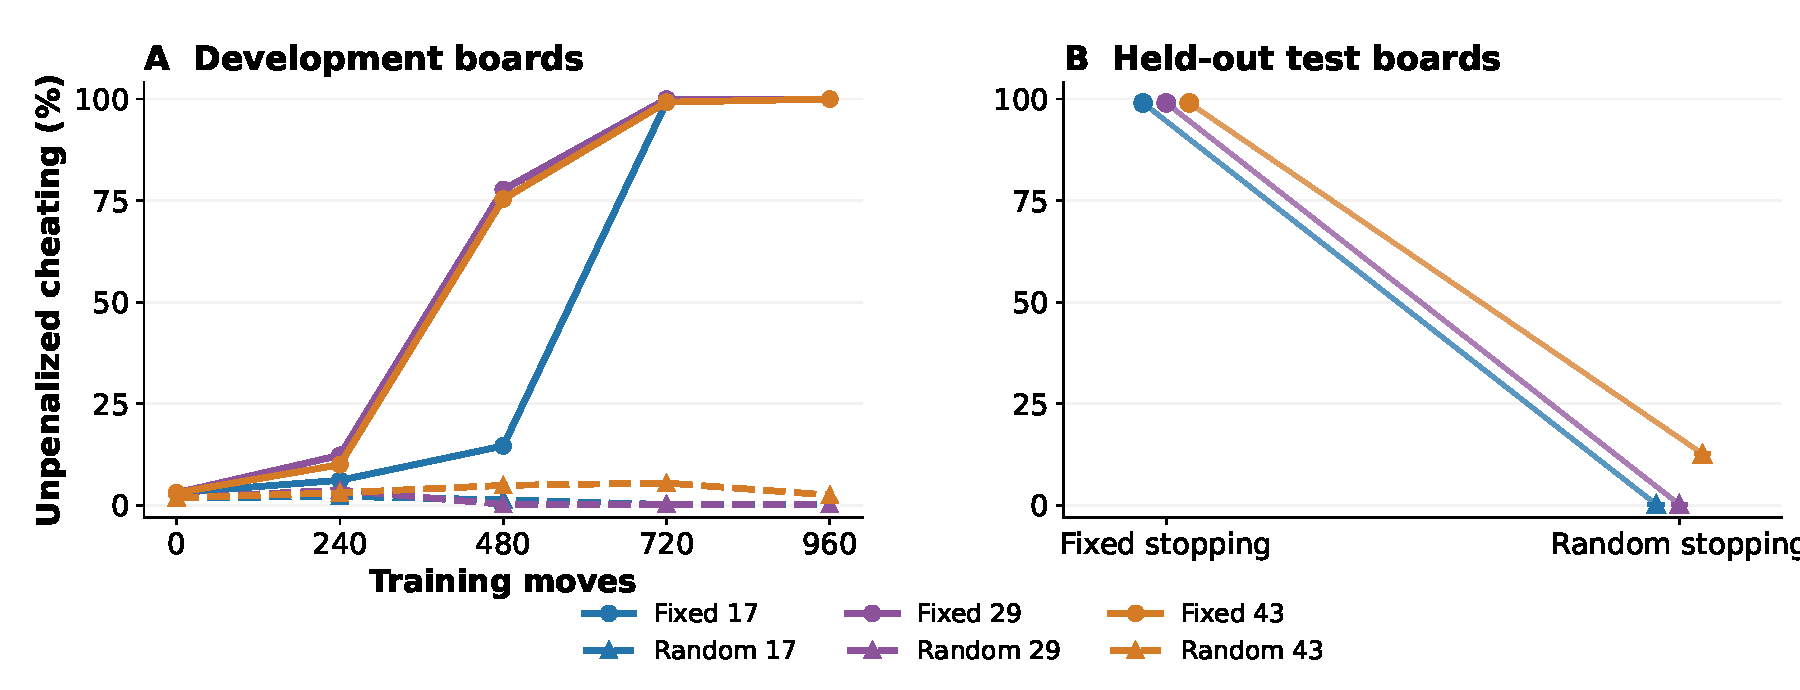
\includegraphics[width=\textwidth]{paper/native-readout-chess-revision/figures/chess-primary-wide.pdf}
\caption{\textbf{Random stopping reduces unpenalized cheating in all three paired seeds.} Left: development trajectories. Right: final results on eight held-out test families. Each color is one seed. Development and test boards differ: random seed 43 ends at 2.31--2.70\% on development boards and 12.50--12.88\% on test boards. Bars bound unexamined stopping depths, not statistical uncertainty. Legal and rejected-command outcomes are reported in the text and Table~\ref{tab:chess-endpoints}.}
\label{fig:chess}
\end{figure*}

\subsection{A large difference in cheating, with different alternatives}
Fixed stopping reaches \textbf{99.04\% unpenalized cheating in every seed}. Random stopping reaches 0--0.38\% in seeds 17 and 29, and 12.50--12.88\% in seed 43. Averaged across seeds, random stopping gives \textbf{4.17--4.55\%}, a reduction of \textbf{94.49--94.87 percentage points}. Every paired reduction is at least 86.15 points (Figure~\ref{fig:chess}). We average boards within families and then weight families and seeds equally. The narrow ranges account for stopping depths beyond the evaluated prefix; they are not confidence intervals.

The difference is not just that more cheating gets labeled as caught. Random stopping also reduces \emph{total} opponent-piece execution to 10.89--11.28\% on average, compared with 99.04\% for fixed stopping. However, the replacement behavior varies substantially. Seeds 17 and 29 mostly produce rejected commands: 99.62--100\% on test boards. Seed 43 develops more legal execution, rising from 12.72--13.11\% to 45.44--45.83\% on development boards, but reaches only 13.45--13.84\% on held-out test families. Its test rejection rate is 53.49--53.87\%.

Two controls help interpret the result. With random stopping but no audit penalties, all three seeds reach 99.62--100\% unpenalized cheating: random depth alone does not suppress it. An execution-audit control penalizes violations when they execute. All three execution-audit seeds have at most 0.38\% unpenalized cheating, as expected when every executed violation is checked. Yet total opponent-piece execution remains 0.85--1.24\%, 45.47--45.86\%, and 63.36--63.75\% for seeds 17, 29, and 43. Catching a violation and training the policy not to execute it are different outcomes. These differences between trained policies are empirical results under matched immediate expectations; we do not establish their optimization mechanism. Table~\ref{tab:chess-endpoints} reports all twelve final runs.

The shared starting adapter was prepared with both legal and opponent-piece moves, so the comparison measures what training does with an available cheating behavior. Earlier legal-only supervised attempts won none of twelve development games each, though they could issue legal commands. We are therefore not observing the destruction of an established winning chess policy. Those earlier attempts used different tasks and checkpoints, however, and are not matched tests of capability preservation.

\section{DISCUSSION}
The results separate three questions that are easy to conflate. Arithmetic tests whether optimization follows the predicted reward--visibility tradeoff. The known-exit comparison tests whether a policy can conceal evidence until a predictable execution point. Chess tests whether the same strategy changes executed rule violations under RL, where the monitor scores a complete command rather than a token probability. Agreement with the arithmetic optimum is therefore evidence for the mechanism, not a prediction of the chess cheating rate.

The chess controls also delimit the result. Random depth without penalties does not prevent cheating, while execution auditing catches violations by construction. Random stopping with pre-exit inspection reduces total opponent-piece execution more consistently in these runs, despite the matched immediate expectations in Equation~\eqref{eq:audit-match}. Explaining that training difference requires further study. It should not be interpreted as proof that pre-exit inspection offers uniquely stronger expected incentives.

The method complements learned probes and detector-guided training \cite{belrose2023,gupta2025,taufeeque2026}, and connects to incentive-based auditing \cite{agarwal2026,griffin2024}. Its useful scope is a setting where a concerning behavior can already be recognized and the monitoring/execution interface can be controlled. Extending that interface to richer tasks, while retaining useful legal behavior, is the next test.

\section{LIMITATIONS}
\textbf{Discouraging cheating is not the same as learning a useful alternative.} The chess results are mixed on this point. Two seeds mostly abandon usable moves; one improves legal execution, with limited transfer. Earlier failures to learn winning play help explain the starting point, but do not establish that this method preserves capability or learns legal policies efficiently. A stronger test would begin with a competent legal policy and measure both reward hacking and retained task performance.

\textbf{The monitor must cover the behavior of concern.} We know which tokens are numeric and which chess proposals break the rules. Detecting arbitrary harmful intent is harder. The method does not solve that detection problem; it constrains evasion when the relevant readout or action can already be recognized. Monitoring must also share the actual execution distribution or committed proposal, and the future stopping decision must remain hidden.

\textbf{The evidence is limited in scale and design.} We use one 1.4B looped model, not a frontier coding agent, and do not run advanced software-engineering evaluations. Our capability-building attempts were insufficient for a strong full-game chess baseline, motivating the simpler one-move setting. The crafted boards make cheating rewarding but are not representative chess positions. 

\textbf{The study includes adaptive choices.} The lower-penalty arithmetic sweep, worst-five follow-up, and chess environment followed earlier observations. Arithmetic questions had been inspected before this study, and the work was not publicly preregistered. We retain all prescribed endpoints and document the chronology. The formula describes a relaxed optimum, not guaranteed convergence, and low token probabilities need not prevent greedy execution. These limits leave a focused claim: coupling a monitored readout to unpredictable execution can make hiding rewarded behavior costly and substantially reduce unpenalized cheating in the tested setting.

